\documentclass[journal,12pt,onecolumn]{IEEEtran}
\usepackage{cite}
 \usepackage{caption}
\usepackage{graphicx}
\usepackage{amsmath,amssymb,amsfonts,amsthm}
\usepackage{algorithmic}
\usepackage{graphicx}
\usepackage{textcomp}
\usepackage{xcolor}
\usepackage{txfonts}
\usepackage{listings}
\usepackage{enumitem}
\usepackage{mathtools}
\usepackage{gensymb}
\usepackage{comment}
\usepackage[breaklinks=true]{hyperref}
\usepackage{tkz-euclide} 
\usepackage{listings}
\usepackage{gvv}                                        
%\def\inputGnumericTable{}                                 
\usepackage[latin1]{inputenc} 
\usetikzlibrary{arrows.meta, positioning}
\usepackage{xparse}
\usepackage{color}                                            
\usepackage{array}                                            
\usepackage{longtable}                                       
\usepackage{calc}                                             
\usepackage{multirow}
\usepackage{multicol}
\usepackage{hhline}                                           
\usepackage{ifthen}                                           
\usepackage{lscape}
\usepackage{tabularx}
\usepackage{array}
\usepackage{float}
\newtheorem{theorem}{Theorem}[section]
\newtheorem{problem}{Problem}
\newtheorem{proposition}{Proposition}[section]
\newtheorem{lemma}{Lemma}[section]
\newtheorem{corollary}[theorem]{Corollary}
\newtheorem{example}{Example}[section]
\newtheorem{definition}[problem]{Definition}
\newcommand{\BEQA}{\begin{eqnarray}}
\newcommand{\EEQA}{\end{eqnarray}}
\usepackage{float}
\graphicspath{{./figs/}}
%\newcommand{\define}{\stackrel{\triangle}{=}}
\theoremstyle{remark}
\usepackage{circuitikz}
\captionsetup{justification=centering}
\usepackage{tikz}
\title{EC: ELECTRONICS AND COMMUNICATION ENGINEERING - 2025}
\author{EE25BTECH11037 - Divyansh}


\begin{document}
\maketitle
\begin{enumerate}

\item If `$\rightarrow$' denotes increasing order of intensity, then the meaning of the words \sbrak{charm $\rightarrow$ enamor $\rightarrow$ bewitch} is analogous to [bored $\rightarrow$ weary].
\hfill{\brak{\text{GATE EC 2025}}}
\begin{multicols}{4}
    \begin{enumerate}
    \item jaded
    \item baffled
    \item dead
    \item worsted
\end{enumerate}
\end{multicols}

\item P, Q, R, S, and T have launched a new startup. Two of them are siblings. The office of the startup has just three rooms. All of them agree that the siblings should not share the same room. 

If S and Q are single children, and the room allocations shown below in $\figref{fig:q2}$ are acceptable to all.
\begin{figure}[H]
    \centering
    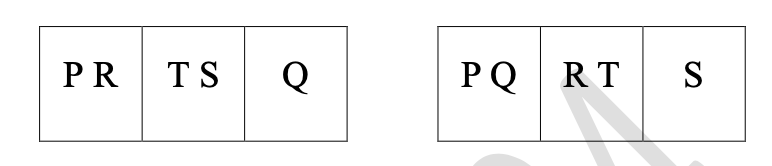
\includegraphics[width=0.5\columnwidth]{q2.png}
    \caption{For q-2}
    \label{fig:q2}
\end{figure}
then, which one of the given options is the siblings?
\hfill{\brak{\text{GATE EC 2025}}}
\begin{multicols}{4}
\begin{enumerate}
    \item P and T
    \item P and S
    \item T and Q
    \item T
\end{enumerate}
\end{multicols}

\item Five years ago, the ratio of Aman's age to his father's age was $1\colon4$, and five years from now, the ratio will be $2\colon5$. What was his father's age when Aman was born?
\hfill{\brak{\text{GATE EC 2025}}}
\begin{multicols}{4}
\begin{enumerate}
    \item 28 years
    \item 30 years
    \item 35 years
    \item 32 years
\end{enumerate}
\end{multicols}

\item For a real number $x>1$,
\begin{align*}
\dfrac{1}{\log_{2}x}+\dfrac{1}{\log_{3}x}+\dfrac{1}{\log_{4}x}=1
\end{align*}
\hfill{\brak{\text{GATE EC 2025}}}

\item The greatest prime factor of $\brak{3^{199}-3^{196}}$ is \underline{\hspace{2cm}}.
\hfill{\brak{\text{GATE EC 2025}}}
\begin{multicols}{4}
\begin{enumerate}
    \item 13
    \item 17
    \item 3
    \item 11
\end{enumerate}
\end{multicols}

\item Sequence the following sentences \brak{P, Q, R, S} in a coherent passage:
\begin{enumerate}[start=16, label=\Alph*:]
    \item Shifu's student exclaimed, "Why do you run since the bull is an illusion?"
    \item Shifu said, "Surely my running away from the bull is also an illusion."
    \item Shifu once proclaimed that all life is illusion.
    \item One day, when a bull gave him chase, Shifu began running for his life.
\end{enumerate}
\hfill{\brak{\text{GATE EC 2025}}}
\begin{multicols}{4}
\begin{enumerate}
    \item SPRQ
    \item SRPQ
    \item RSPQ
    \item RSQP
\end{enumerate}
\end{multicols}

\item Four identical cylindrical chalk-sticks, each of radius $r=0.5$ cm and length $l=10$ cm, are bound tightly together using a duct tape as shown in the following $\figref{fig:q7}$. The width of the duct tape is equal to the length of the chalk-stick. The area \brak{in cm$^2$} of the duct tape required to wrap the bundle of chalk-sticks once, is \underline{\hspace{2cm}}.
\begin{figure}[H]
    \centering
    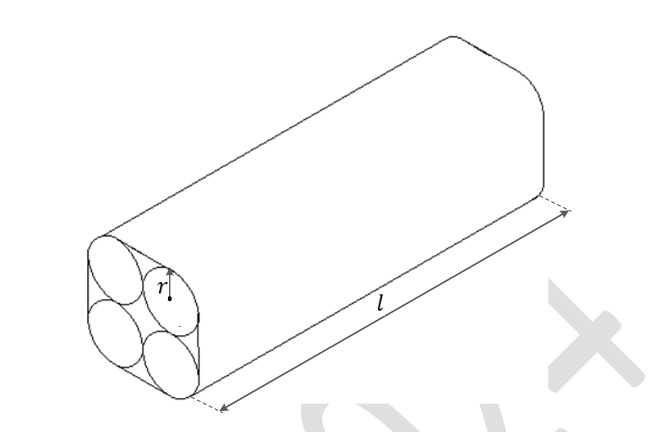
\includegraphics[width=0.5\columnwidth]{q7.png}
    \caption{For q-7}
    \label{fig:q7}
\end{figure}
\hfill{\brak{\text{GATE EC 2025}}}
\begin{multicols}{2}
\begin{enumerate}
    \item $20\brak{4+\pi}$
    \item $20\brak{8+\pi}$
    \item $10\brak{8+\pi}$
    \item $10\brak{4+\pi}$
\end{enumerate}
\end{multicols}

\item The bar chart shows the data for the percentage of population falling into different categories based on Body Mass Index \brak{BMI} in 2003 and 2023.
\begin{figure}[H]
    \centering
    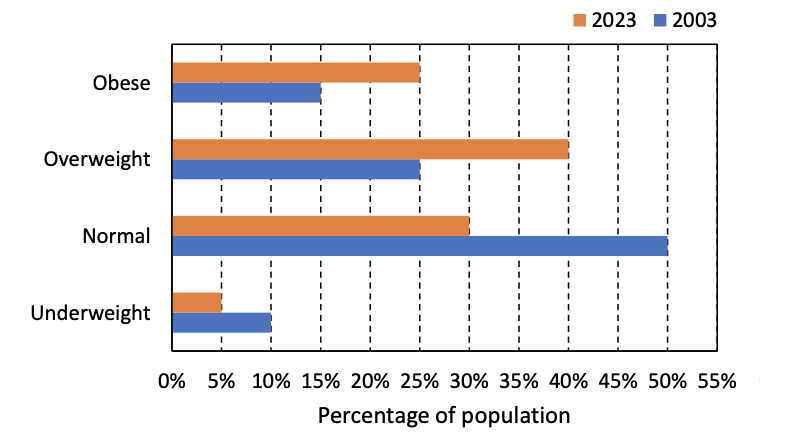
\includegraphics[width=0.8\columnwidth]{q8.png}
    \caption{For q-8}
    \label{fig:q8}
\end{figure}
Based on the data provided, which one of the following options is INCORRECT?
\hfill{\brak{\text{GATE EC 2025}}}
\begin{enumerate}
    \item The ratio of the percentage of population falling into overweight category to the percentage of population falling into normal category has increased in 20 years.
    \item The ratio of the percentage of population falling into underweight category to the percentage of population falling into normal category has decreased in 20 years.
    \item The ratio of the percentage of population falling into obese category to the percentage of population falling into normal category has decreased in 20 years.
    \item The percentage of population falling into normal category has decreased in 20 years.
\end{enumerate}

\item Examples of mirror and water reflections are shown in the figures below:
\begin{figure}[H]
    \centering
    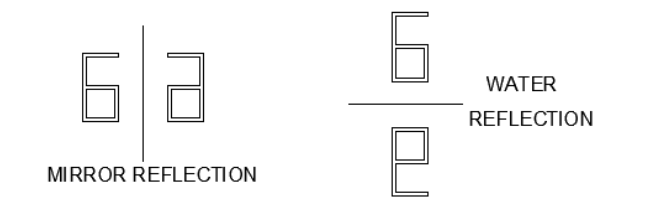
\includegraphics[width=0.7\columnwidth]{q91.png}
    \caption{For q-9}
    \label{fig:q9}
\end{figure}
An object appears as the following image after first reflecting in a mirror and then reflecting on water.
\begin{figure}[H]
    \centering
    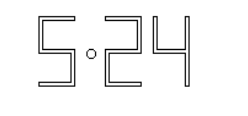
\includegraphics[width=0.3\columnwidth]{q92.png}
    \caption*{}
    \label{fig:q9}
\end{figure}
The original object is \underline{\hspace{2cm}}.
\hfill{\brak{\text{GATE EC 2025}}}
\begin{multicols}{2}
\begin{enumerate}
    \item 
\includegraphics[width=0.3\columnwidth]{q9a.png}
    \item 
\includegraphics[width=0.3\columnwidth]{q9b.png}
    \item 
\includegraphics[width=0.3\columnwidth]{q9c.png}
    \item 
\includegraphics[width=0.3\columnwidth]{q9d.png}
\end{enumerate}
\end{multicols}

\item Two identical sheets A and B, of dimensions $24 \text{ cm} \times 16$ cm, can be folded into half using two distinct operations, FO1 or FO2. In FO1, the axis of folding remains parallel to the initial long edge, and in FO2, the axis of folding remains parallel to the initial short edge. If sheet A is folded twice using FO1, and sheet B is folded twice using FO2, the ratio of the perimeters of the final shapes of A and B is \underline{\hspace{2cm}}.
\hfill{\brak{\text{GATE EC 2025}}}
\begin{multicols}{2}
\begin{enumerate}
    \item $14:11$
    \item $11:14$
    \item $18:11$
    \item $11:18$
\end{enumerate}
\end{multicols}

\item The general form of the complementary function of a differential equation is given by $y\brak{t}=\brak{At+B}e^{-2t}$, where A and B are real constants determined by the initial condition. The corresponding differential equation is \underline{\hspace{2cm}}.
\hfill{\brak{\text{GATE EC 2025}}}
\begin{enumerate}
    \item $\dfrac{d^{2}y}{dt^{2}}+4\dfrac{dy}{dt}+4y=f\brak{t}$
    \item $\dfrac{d^{2}y}{dt^{2}}+4y=f\brak{t}$
    \item $\dfrac{d^{2}y}{dt^{2}}+3\dfrac{dy}{dt}+2y=f\brak{t}$
    \item $\dfrac{d^{2}y}{dt^{2}}+5\dfrac{dy}{dt}+6y=f\brak{t}$
\end{enumerate}

\item In the context of Bode magnitude plots, 40 dB/decade is the same as \underline{\hspace{2cm}}.
\hfill{\brak{\text{GATE EC 2025}}}
\begin{multicols}{2}
\begin{enumerate}
    \item $12 dB/octave$
    \item $6 dB/octave$
    \item $20 dB/octave$
    \item $10 dB/octave$
\end{enumerate}
\end{multicols}

\item In the feedback control system shown in the $\figref{fig:q13}$ below, $R\brak{s}$, $E\brak{s}$ and $Y\brak{s}$ are the Laplace transforms of $r\brak{t}$, $e\brak{t}$ and $y\brak{t}$ respectively. If the input is a unit step function, then $\lim_{t \to \infty} e\brak{t}$ is \underline{\hspace{2cm}}.
\begin{figure}[H]
    \centering
    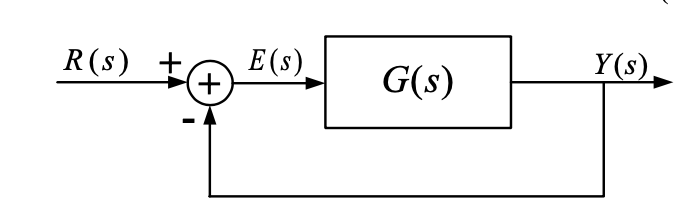
\includegraphics[width=0.5\columnwidth]{q13.png}
    \caption{For q-13}
    \label{fig:q13}
\end{figure}
\hfill{\brak{\text{GATE EC 2025}}}
\begin{multicols}{2}
  \begin{enumerate}
    \item $0$
    \item $1$
    \item $0.5$
    \item does not exist, is oscillatory
\end{enumerate}  
\end{multicols}


\item A digital communication system transmits through a noiseless bandlimited channel $\sbrak{-W, W}$. The received signal at the output of the receiving filter is given by $y\brak{t} = \sum_{k} a_k p\brak{t - kT}$, where $a_k$ are the symbols and $p\brak{t}$ is the overall system response to a single symbol. The received signal is sampled at $t = mT$. The Fourier transform of $p\brak{t}$ is $P\brak{f}$. The Nyquist condition that $P\brak{f}$ must satisfy for zero intersymbol interference at the receiver is \underline{\hspace{2cm}}.
\hfill{\brak{\text{GATE EC 2025}}}
\begin{enumerate}
    \item $\sum_{m=-\infty}^{\infty} P\brak{f-\dfrac{m}{T}} = T, \text{ for } \abs{f} \leq W$
    \item $\sum_{m=-\infty}^{\infty} P\brak{f-\dfrac{m}{T}} = T, \text{ for } \abs{f} \leq \dfrac{1}{2T}$
    \item $P\brak{f} = T, \text{ for } \abs{f} \leq W$
    \item $P\brak{f} = T, \text{ for } \abs{f} \leq \dfrac{1}{2T}$
\end{enumerate}

\item Consider a lossless transmission line terminated with a short circuit as shown in the $\figref{fig:q15}$ below. As one moves towards the generator from the load, the normalized impedances, $z_1, z_2, z_3$ and $z_4$ \brak{indicated in the figure} are \underline{\hspace{2cm}}.
\begin{figure}[H]
    \centering
    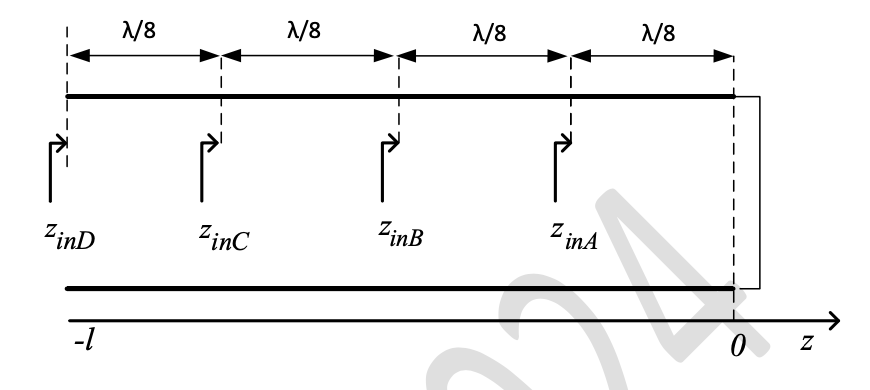
\includegraphics[width=0.7\columnwidth]{q15.png}
    \caption{For q-15}
    \label{fig:q15}
\end{figure}
\hfill{\brak{\text{GATE EC 2025}}}
\begin{enumerate}
    \item $z_1 = +1j \ohm , z_2 = \infty , z_3 = -1j \ohm , z_4 = 0$
    \item $z_1 = \infty , z_2 = +0.4j \ohm , z_3 = 0 , z_4 = +0.4j \ohm$
    \item $z_1 = -1j \ohm , z_2 = 0, z_3 = +1j \ohm , z_4 = \infty$
    \item $z_1 = +0.4j \ohm , z_2 = \infty, z_3 = -0.4j \ohm , z_4 = 0$
\end{enumerate}

\item Let $\hat{x}$ and $\hat{y}$ be the unit vectors along $x$ and $y$ axes, respectively and let $\alpha$ be a positive constant. Which one of the following statements is true for the vector fields $\vec{F_1} = \alpha\brak{y\hat{x} - x\hat{y}}$ and $\vec{F_2} = \alpha\brak{y\hat{x} + x\hat{y}}$?
\hfill{\brak{\text{GATE EC 2025}}}
\begin{multicols}{2}
    \begin{enumerate}
    \item Both $\vec{F_1}$ and $\vec{F_2}$ are electrostatic fields.
    \item Only $\vec{F_1}$ is an electrostatic field.
    \item Only $\vec{F_2}$ is an electrostatic field.
    \item Neither $\vec{F_1}$ nor $\vec{F_2}$ is an electrostatic field.
\end{enumerate}
\end{multicols}


\item In the circuit shown below in the $\figref{fig:q17}$, assume that the long channel NMOS transistor is biased in saturation. The small signal trans-conductance of the transistor is $g_m$. Neglect body effect, channel length modulation and intrinsic device capacitances. The small signal input impedance $Z_{in}$ is \underline{\hspace{2cm}}.
\begin{figure}[H]
    \centering
    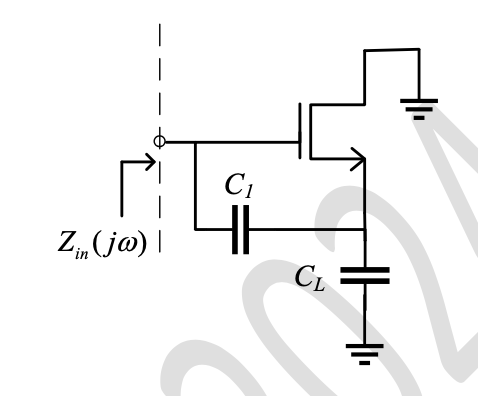
\includegraphics[width=0.4\columnwidth]{q17.png}
    \caption{For q-17}
    \label{fig:q17}
\end{figure}
\hfill{\brak{\text{GATE EC 2025}}}
\begin{multicols}{4}
    \begin{enumerate}
    \item $R_S$
    \item $\dfrac{1}{g_m}$
    \item $R_S + \dfrac{1}{g_m}$
    \item $R_S || \dfrac{1}{g_m}$
\end{enumerate}
\end{multicols}


\item For the closed loop amplifier circuit shown below in the $\figref{fig:q-18}$, the magnitude of open loop low frequency small signal voltage gain is 40. All the transistors are biased in saturation. The current source $I_{SS}$ is ideal. Neglect body effect, channel length modulation and intrinsic device capacitances. The closed loop low frequency small signal voltage gain $v_{out}/v_{in}$ \brak{rounded off to three decimal places} is \underline{\hspace{2cm}}.
\begin{figure}[H]
    \centering
    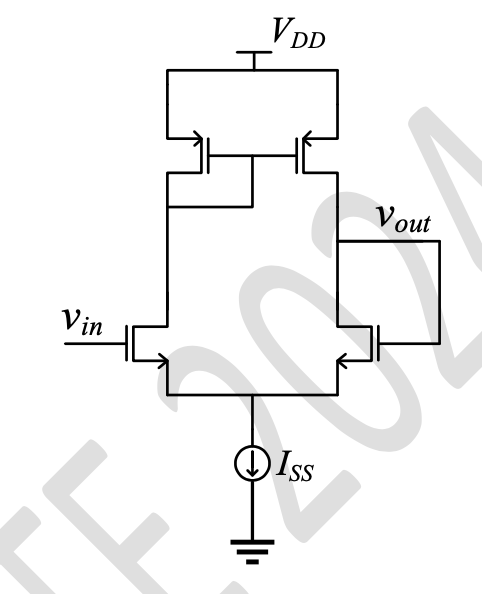
\includegraphics[width=0.3\columnwidth]{q18.png}
    \caption{For q-18}
    \label{fig:q18}
\end{figure}
\hfill{\brak{\text{GATE EC 2025}}}

\item For the Boolean function $F\brak{A, B, C,D} = \sum m\brak{0,2,5,7,8,10,12,13,14,15}$, the essential prime implicants are \underline{\hspace{2cm}}.
\hfill{\brak{\text{GATE EC 2025}}}
\begin{multicols}{4}
\begin{enumerate}
    \item $BD, \bar{B}\bar{D}$
    \item $BD, A\bar{B}$
    \item $A\bar{B}, \bar{B}\bar{D}$
    \item $BD, \bar{B}\bar{D}, A\bar{C}$
\end{enumerate}
\end{multicols}

\item A white Gaussian noise with zero mean and power spectral density $N_0/2$, when applied to a first-order RC low pass filter produces an output $n\brak{t}$. At a particular time $t = t_k$, the variance of the random variable $n\brak{t_k}$ is \underline{\hspace{2cm}}.
\hfill{\brak{\text{GATE EC 2025}}}
\begin{multicols}{4}
    \begin{enumerate}
    \item $\dfrac{N_0}{4RC}$
    \item $\dfrac{N_0}{2RC}$
    \item $\dfrac{N_0}{RC}$
    \item $\dfrac{N_0}{2}$
\end{enumerate}
\end{multicols}


\item A causal and stable LTI system with impulse response $h\brak{t}$ produces an output $y\brak{t}$ for an input signal $x\brak{t}$. A signal $x\brak{0.5t}$ is applied to another causal and stable LTI system with impulse response $h\brak{0.5t}$. The resulting output is \underline{\hspace{2cm}}.

\hfill{\brak{\text{GATE EC 2025}}}
\begin{multicols}{4}
\begin{enumerate}
    \item $2y\brak{0.5t}$
    \item $4y\brak{0.5t}$
    \item $0.25y\brak{2t}$
    \item $0.25y\brak{0.25t}$
\end{enumerate}
\end{multicols}

\item For non-degenerately doped n-type silicon, which one of the following plots represents the temperature \brak{$T$} dependence of free electron concentration \brak{$n$}.
\hfill{\brak{\text{GATE EC 2025}}}
\begin{figure}[H]
\centering
\begin{minipage}{0.45\textwidth}
    \centering
    (A) 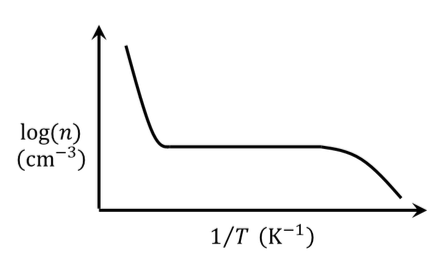
\includegraphics[width=0.9\linewidth]{q22a.png}
\end{minipage}
\begin{minipage}{0.45\textwidth}
    \centering
    (B) 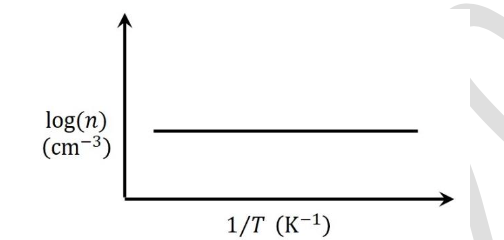
\includegraphics[width=0.9\linewidth]{q22b.png}
\end{minipage}
\begin{minipage}{0.45\textwidth}
    \centering
    (C) 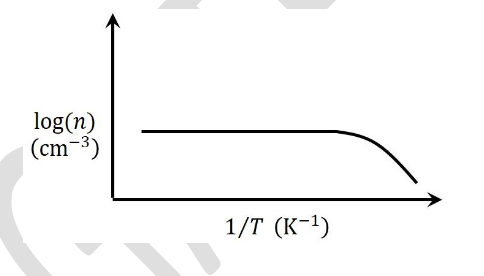
\includegraphics[width=0.9\linewidth]{q22c.png}
\end{minipage}
\begin{minipage}{0.45\textwidth}
    \centering
    (D) 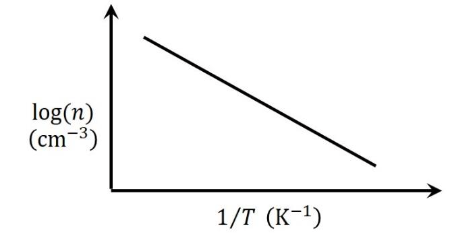
\includegraphics[width=0.9\linewidth]{q22d.png}
\end{minipage}
\caption*{}
\label{fig:q22}
\end{figure}

\item In the circuit shown in the $\figref{fig:q23}$, the $n \colon 1$ step-down transformer and the diodes are ideal. The diodes have no voltage drop in forward biased condition. If the input voltage \brak{in Volts} is $V_s\brak{t} = 10\sin\omega t$ and the average value of load voltage $V_L\brak{t}$ \brak{in Volts} is $2.5/\pi$, the value of $n$ is \underline{\hspace{2cm}}.
\begin{figure}[H]
    \centering
    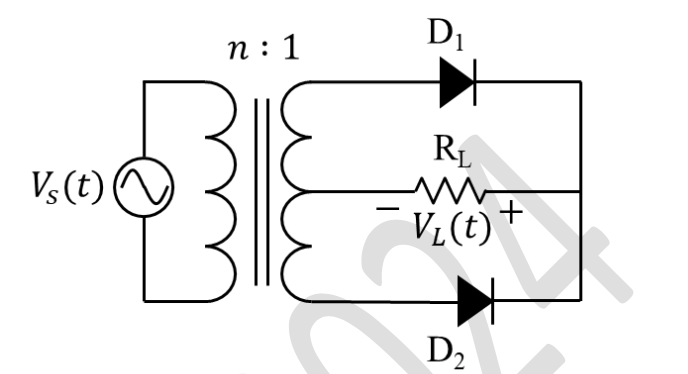
\includegraphics[width=0.5\columnwidth]{q23.png}
    \caption{For q-23}
    \label{fig:q23}
\end{figure}
\hfill{\brak{\text{GATE EC 2025}}}
\begin{multicols}{4}
\begin{enumerate}
    \item 4
    \item 8
    \item 12
    \item 16
\end{enumerate}
\end{multicols}

\item For a causal discrete-time LTI system with transfer function $H\brak{z} = \dfrac{2z^2+3}{\brak{z + \dfrac{1}{3}}\brak{z - \dfrac{1}{3}}}$ which of the following statements is/are true?

\hfill{\brak{\text{GATE EC 2025}}}
\begin{multicols}{2}
\begin{enumerate}
    \item The system is stable.
    \item The system is a minimum phase system.
    \item The initial value of the impulse response is 2.
    \item The final value of the impulse response is 0.
\end{enumerate}    
\end{multicols}


\item Let $\rho\brak{\vec{r},t}$ and $\vec{v}\brak{\vec{r},t}$ represent density and velocity, respectively, at a point $\vec{r}$ and time $t$. Assume $\rho\brak{\vec{r},t}$ is continuous. Let $V$ be an arbitrary volume in space enclosed by the closed surface $S$ and $\hat{n}$ be the outward unit normal of $S$. Which of the following equations is/are equivalent to $\dfrac{\partial \rho}{\partial t} + \nabla \cdot \brak{\rho \vec{v}} = 0$?

\hfill{\brak{\text{GATE EC 2025}}}
\begin{multicols}{2}
 \begin{enumerate}
    \item $\dfrac{d}{dt} \int_V \rho dV = - \oint_S \rho \vec{v} \cdot \hat{n} dS$
    \item $\dfrac{\partial}{\partial t} \int_V \rho dV = - \oint_S \rho \vec{v} \cdot d\vec{S}$
    \item $\dfrac{\partial \rho}{\partial t} + \rho \nabla \cdot \vec{v} + \vec{v} \cdot \nabla \rho = 0$
    \item $\dfrac{\partial \rho}{\partial t} + \rho \nabla \cdot \vec{v} = 0$
\end{enumerate}   
\end{multicols}

\item The free electron concentration profile n(x) in a doped semiconductor at equilibrium is shown in the $\figref{fig:q26}$, where the points A, B, and C mark three different positions. Which of the following statements is/are true?
\begin{figure}[H]
    \centering
    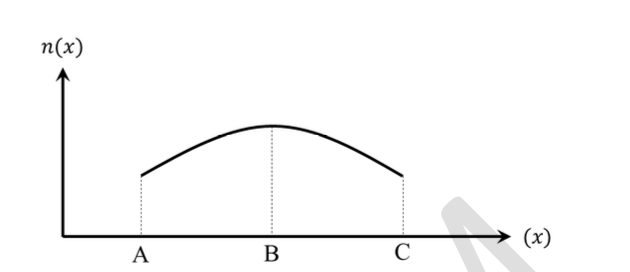
\includegraphics[width=0.5\columnwidth]{q26.png}
    \caption{For q-26}
    \label{fig:q26}
\end{figure}
\hfill{\brak{\text{GATE EC 2025}}}
\begin{enumerate}
    \item For $x$ between B and C, the electron diffusion current is directed from C to B.
    \item For $x$ between B and A, the electron drift current is directed from B to A.
    \item For $x$ between B and C, the electric field is directed from B to C.
    \item For $x$ between B and A, the electric field is directed from A to B.
\end{enumerate}

\item A machine has a 32-bit architecture with 1-word long instructions. It has 24 registers and supports an instruction set of size 40. Each instruction has five distinct fields, namely opcode, two source register identifiers, one destination register identifier, and an immediate value. Assuming that the immediate operand is an unsigned integer, its maximum value is \underline{\hspace{2cm}}.

\hfill{\brak{\text{GATE EC 2025}}}

\item An amplitude modulator has output \brak{in Volts} $s\brak{t} = A\cos\brak{2\pi f_c t} + B \cos\brak{2\pi f_m t}\cos\brak{2\pi f_c t}$. The carrier power normalized to 1 $\ohm$ resistance is 50 Watts. The ratio of the total sideband power to the total power is 1/9. The value of $B$ \brak{\text{in Volts, rounded off to two decimal places}} is \underline{\hspace{2cm}}.

\hfill{\brak{\text{GATE EC 2025}}}

\item In a number system of base $r$, the equation $x^2 - 12x + 37 = 0$ has $x = 8$ as one of its solutions. The value of $r$ is \underline{\hspace{2cm}}.

\hfill{\brak{\text{GATE EC 2025}}}

\item Let $\mathbb{R}$ and $\mathbb{R}^3$ denote the set of real numbers and the three dimensional vector space over it, respectively. The value of $\alpha$ for which the set of vectors $\{[2, -3, \alpha], [3, -1, 3], [1, -5, 7]\}$ does not form a basis of $\mathbb{R}^3$ is \underline{\hspace{2cm}}.

\hfill{\brak{\text{GATE EC 2025}}}

\item In the given circuit, the current $I_x$ \brak{in \ mA} is \underline{\hspace{2cm}}.
\begin{figure}[H]
    \centering
    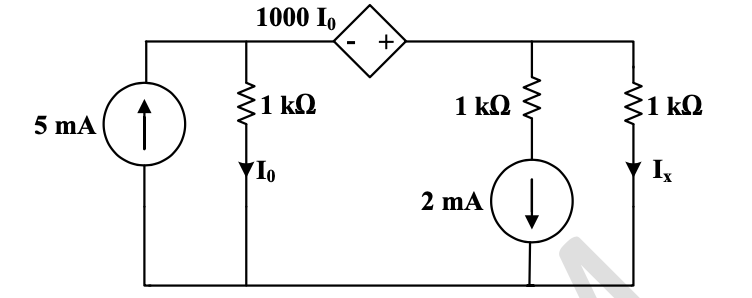
\includegraphics[width=0.5\columnwidth]{q31.png}
    \caption{For q-31}
    \label{fig:q31}
\end{figure}
\hfill{\brak{\text{GATE EC 2025}}}

\item In the circuit given below in $\figref{fig:q32}$, the switch S was kept open for a sufficiently long time and is closed at time $t = 0$. The time constant \brak{in seconds} of the circuit for $t > 0$ is \underline{\hspace{2cm}}.
\begin{figure}[H]
    \centering
    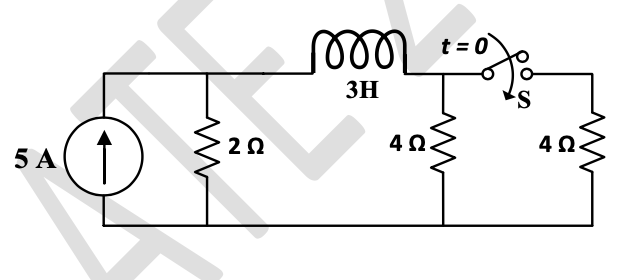
\includegraphics[width=0.5\columnwidth]{q32.png}
    \caption{For q-32}
    \label{fig:q32}
\end{figure}
\hfill{\brak{\text{GATE EC 2025}}}

\item Suppose $X_1$ and $X_2$ are independent and identically distributed random variables that are distributed uniformly in the interval $[0, 1]$. The probability that $\max\brak{X_1, X_2} > 1/2$ is \underline{\hspace{2cm}}.
\hfill{\brak{\text{GATE EC 2025}}}

\item A source transmits symbols from an alphabet of size 16. The value of maximum achievable entropy \brak{in bits} is \underline{\hspace{2cm}}.
\hfill{\brak{\text{GATE EC 2025}}}

\item As shown in the circuit below in the $\figref{fig:q35}$, the initial voltage across the capacitor is 10 V, with the switch being open. The switch is then closed at $t = 0$. The total energy dissipated in the ideal Zener diode \brak{$V_Z = 5$ V} after the switch is closed \brak{in mJ, rounded off to three decimal places} is \underline{\hspace{2cm}}.
\begin{figure}[H]
    \centering
    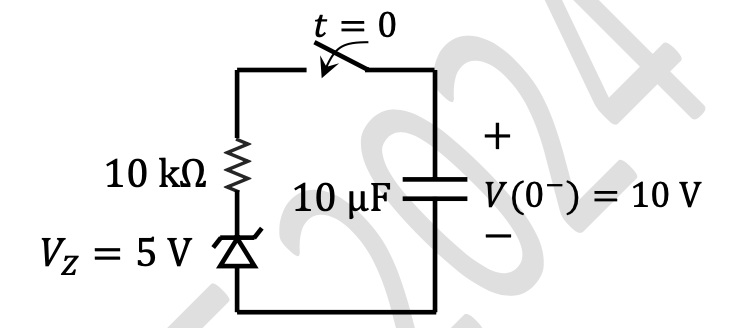
\includegraphics[width=0.5\columnwidth]{q35.png}
    \caption{For q-35}
    \label{fig:q35}
\end{figure}
\hfill{\brak{\text{GATE EC 2025}}}

\item Consider the Earth to be a perfect sphere of radius R. Then the surface area of the region, enclosed by the 60$\degree$N latitude circle, that contains the north pole in its interior is \underline{\hspace{2cm}}.

\hfill{\brak{\text{GATE EC 2025}}}
\begin{multicols}{4}
    \begin{enumerate}
    \item $\pi R^2$
    \item $2\pi R^2$
    \item $\dfrac{\pi R^2}{2}$
    \item $4\pi R^2$
\end{enumerate}
\end{multicols}


\item Consider a unity negative feedback control system with forward path gain $G\brak{s} = \dfrac{K}{s\brak{s+a}}$. The impulse response of the closed-loop system decays faster than $e^{-t}$ if \underline{\hspace{2cm}}.
\hfill{\brak{\text{GATE EC 2025}}}
\begin{multicols}{4}
    \begin{enumerate}
    \item $a > 2$
    \item $a < 2$
    \item $K > a/2$
    \item $K < a/2$
\end{enumerate}
\end{multicols}


\item A satellite attitude control system, as shown below in $\figref{fig:q38}$, has a plant with transfer function $G\brak{s} = \dfrac{1}{s^2}$ cascaded with a compensator $C\brak{s} = K\dfrac{s+\alpha}{s+1}$, where $K$ and $\alpha$ are positive real constants. In order for the closed-loop system to have poles at $-1 \pm j\sqrt{3}$, the value of $\alpha$ must be \underline{\hspace{2cm}}.
\begin{figure}[H]
    \centering
    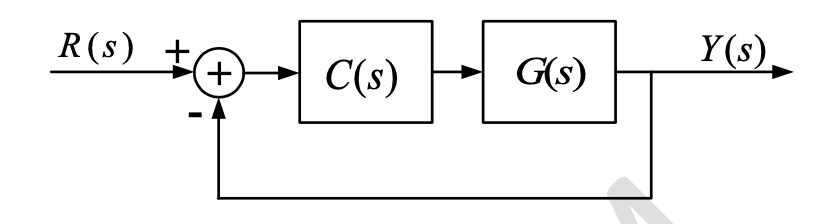
\includegraphics[width=0.5\columnwidth]{q38.png}
    \caption{For q-38}
    \label{fig:q38}
\end{figure}
\hfill{\brak{\text{GATE EC 2025}}}
\begin{multicols}{4}
\begin{enumerate}
    \item 0
    \item 1
    \item 2
    \item 3
\end{enumerate}
\end{multicols}

\item A uniform plane wave with electric field $\vec{E} =A_y \hat{a_y } E_0 \cos\brak{\omega t - \beta x}$ V/m is travelling in the air \brak{relative permittivity, $\epsilon_r=1$ and relative permeability, $\mu_r=1$} in the $+x$ direction \brak{$\beta$ is a positive constant, $\hat{y}$ is the unit vector along the $y$ axis}. It is incident normally on an ideal electric conductor \brak{conductivity, $\sigma=\infty$} at $x = 0$. The position of the first null of the total magnetic field in the air \brak{measured from $x = 0$, in metres} is \underline{\hspace{2cm}}.

\hfill{\brak{\text{GATE EC 2025}}}
\begin{multicols}{4}
  \begin{enumerate}
    \item $\dfrac{\pi}{2\beta}$
    \item $\dfrac{\pi}{\beta}$
    \item $\dfrac{2\pi}{\beta}$
    \item $0$
\end{enumerate}  
\end{multicols}

\item A 4-bit priority encoder has inputs $D_3, D_2, D_1$, and $D_0$ in descending order of priority. The two-bit output $AB$ is generated as 00, 01, 10, and 11 corresponding to inputs $D_0, D_1, D_2$, and $D_3$, respectively. \brak{This \ is \ a \ correction\ from\ the\ original\ text\ for\ standard\ priority\ encoder\ logic}. The Boolean expression of the output bit $B$ is \underline{\hspace{2cm}}.
\hfill{\brak{\text{GATE EC 2025}}}
\begin{multicols}{4}
\begin{enumerate}
    \item $\bar{D_3} \bar{D_2}$
    \item $\bar{D_3} D_2 + \bar{D_3} \bar{D_1}$
    \item $D_3 \bar{D_2} + \bar{D_3} D_1$
    \item $\bar{D_3} D_1$
\end{enumerate}
\end{multicols}


\item The propagation delay of the 2 $\times$ 1 MUX shown in the $\figref{fig:q41}$ is $10 ns$. Consider the propagation delay of the inverter as $0 ns$. If S is set to 1 then the output Y is \underline{\hspace{2cm}}.
\begin{figure}[H]
    \centering
    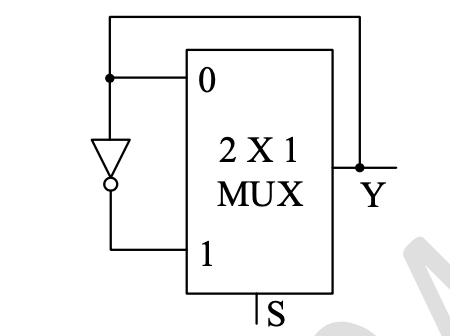
\includegraphics[width=0.4\columnwidth]{q41.png}
    \caption{For q-41}
    \label{fig:q41}
\end{figure}
\hfill{\brak{\text{GATE EC 2025}}}
\begin{multicols}{2}
\begin{enumerate}
    \item a square wave of frequency 100 MHz
    \item a square wave of frequency 50 MHz
    \item constant at 0
    \item constant at 1
\end{enumerate} 
\end{multicols}


\item The sequence of states \brak{$Q_1 Q_0$} of the given synchronous sequential circuit is $\underline{\hspace{2cm}}$.
\begin{figure}[H]
    \centering
    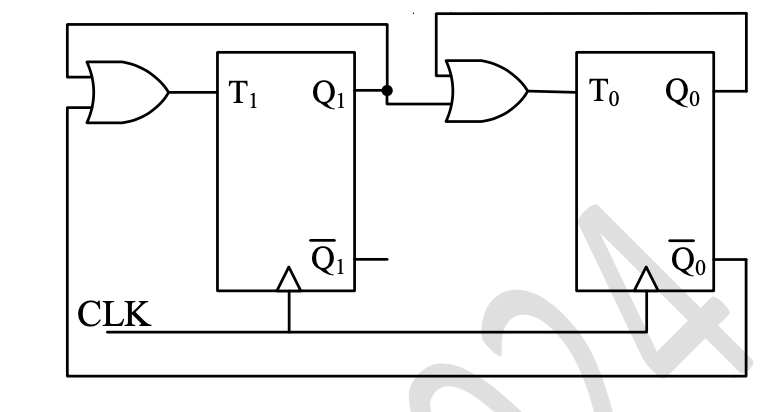
\includegraphics[width=0.6\columnwidth]{q42.png}
    \caption{For q-42}
    \label{fig:q42}
\end{figure}
\hfill{\brak{\text{GATE EC 2025}}}
\begin{enumerate}
    \item $00 \rightarrow 10 \rightarrow 11 \rightarrow 00$
    \item $11 \rightarrow 00 \rightarrow 10 \rightarrow 01 \rightarrow 00$
    \item $01 \rightarrow 10 \rightarrow 11 \rightarrow 00 \rightarrow 01$
    \item $00 \rightarrow 01 \rightarrow 10 \rightarrow 00$
\end{enumerate}

\item Let $z$ be a complex variable. If $f\brak{z} = \dfrac{e^{2z}}{\brak{z+1}^4}$ and $C$ is the circle $\abs{z}=2$ in the complex plane then $\oint_C f\brak{z} dz$ is \underline{\hspace{2cm}}.
\hfill{\brak{\text{GATE EC 2025}}}
\begin{multicols}{4}
    \begin{enumerate}
    \item $\dfrac{8\pi i}{3e^2}$
    \item $\dfrac{8\pi i e^2}{3}$
    \item $\dfrac{16\pi i}{3e^2}$
    \item $\dfrac{16\pi i e^2}{3}$
\end{enumerate}
\end{multicols}

\item Consider two continuous time signals $x\brak{t}$ and $y\brak{t}$ as shown below in $\figref{fig:q44}$. If $X\brak{f}$ denotes the Fourier transform of $x\brak{t}$, then the Fourier transform of $y\brak{t}$ is \underline{\hspace{2cm}}.
\begin{figure}[H]
    \centering
    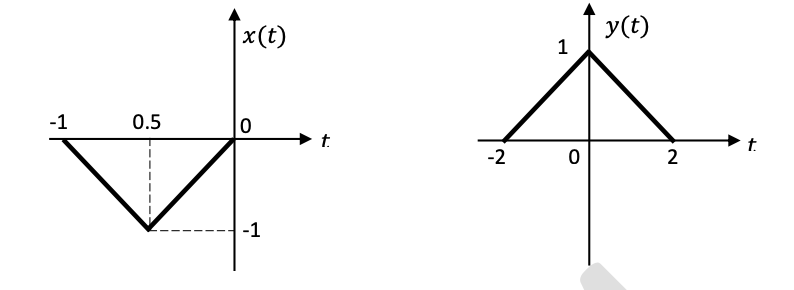
\includegraphics[width=0.6\columnwidth]{q44.png}
    \caption{For q-44}
    \label{fig:q44}
\end{figure}
\hfill{\brak{\text{GATE EC 2025}}}
\begin{multicols}{4}
   \begin{enumerate}
    \item $-4X\brak{4f}e^{-j\pi f}$
    \item $-4X\brak{4f}e^{-j4\pi f}$
    \item $-\dfrac{1}{4}X\brak{f/4}e^{-j\pi f}$
    \item $-\dfrac{1}{4}X\brak{f/4}e^{-j4\pi f}$
\end{enumerate} 
\end{multicols}


\item A source transmits a symbol $S$ taken from $\{+2, -2\}$ with equal probability, over an additive white Gaussian noise channel. The received noisy symbol is given by $R = S + N$ where the noise $N$ is zero mean with variance 4 and is independent of $S$. Using $Q\brak{x} =\dfrac{1}{\sqrt{2\pi}}\int_x^\infty e^{-t^2/2}dt$, the optimum symbol error probability is \underline{\hspace{2cm}}.
\hfill{\brak{\text{GATE EC 2025}}}
\begin{multicols}{4}
    \begin{enumerate}
    \item $Q\brak{0.5}$
    \item $Q\brak{1}$
    \item $Q\brak{2}$
    \item $Q\brak{4}$
\end{enumerate}
\end{multicols}


\item A full scale sinusoidal signal is applied to a 10-bit ADC. The fundamental signal component in the ADC output has a normalized power of 1 W, and the total noise and distortion normalized power is 10 $\mu$W. The effective number of bits \brak{\text{rounded off to the nearest integer}}  of the ADC is \underline{\hspace{2cm}}.

\hfill{\brak{\text{GATE EC 2025}}}
\begin{multicols}{4}
\begin{enumerate}
    \item 7
    \item 8
    \item 9
    \item 10
\end{enumerate}
\end{multicols}

\item The information bit sequence $\{1, 1, 1, 0, 1, 0, 1, 0, 1\}$ is to be transmitted by encoding with Cyclic Redundancy Check 4 \brak{CRC-4} code, for which the generator polynomial is $C\brak{x} = x^4 + x + 1$. The encoded sequence of bits is \underline{\hspace{2cm}}.
\hfill{\brak{\text{GATE EC 2025}}}
\begin{multicols}{2}
\begin{enumerate}
    \item $\brak{1, 1, 1, 0, 1, 0, 1, 0, 1, 1, 1, 0, 0}$
    \item $\brak{1, 1, 1, 0, 1, 0, 1, 0, 1, 1, 1, 0, 1}$
    \item $\brak{1, 1, 1, 0, 1, 0, 1, 0, 1, 1, 1, 1, 0}$
    \item $\brak{1, 1, 1, 0, 1, 0, 1, 0, 1, 0, 1, 0, 0}$
\end{enumerate}
\end{multicols}

\item A continuous time signal $x\brak{t} = 2 \cos\brak{8\pi t + \pi/3}$ is sampled at a rate of $15 Hz$. The sampled signal $x_s\brak{t}$ when passed through an LTI system with impulse response $h\brak{t} = \brak{\dfrac{\sin 2\pi t}{\pi t}} \cos\brak{38\pi t - \pi/2}$ produces an output $x_o\brak{t}$. The expression for $x_o\brak{t}$ is \underline{\hspace{2cm}}.
\hfill{\brak{\text{GATE EC 2025}}}
\begin{multicols}{2}
\begin{enumerate}
    \item $15 \sin\brak{38\pi t + \pi/3}$
    \item $15 \sin\brak{38\pi t - \pi/3}$
    \item $15 \cos\brak{38\pi t - \pi/6}$
    \item $15 \cos\brak{38\pi t + \pi/6}$
\end{enumerate}
\end{multicols}

\item The opamps in the circuit shown in $\figref{fig:q49}$ are ideal, but have saturation voltages of $\pm10$ V. Assume that the initial inductor current is 0 A. The input voltage \brak{$V_i$} is a triangular signal with peak voltages of $\pm2$ V and time period of 8 $\mu$s. Which one of the following statements is true?
\begin{figure}[H]
    \centering
    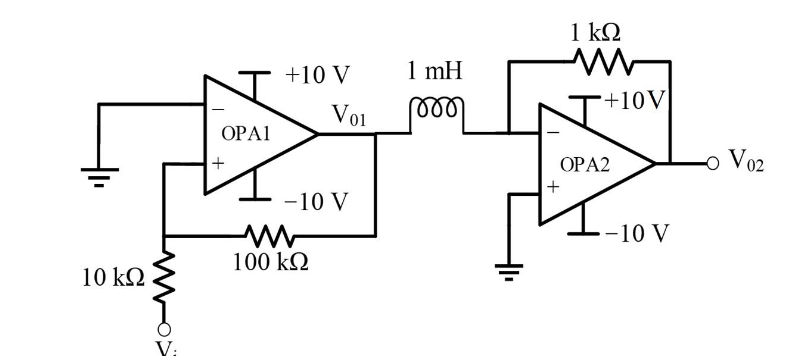
\includegraphics[width=0.6\columnwidth]{q49.png}
    \caption{for q-49}
    \label{fig:q49}
\end{figure}
\hfill{\brak{\text{GATE EC 2025}}}
\begin{enumerate}
    \item $V_{01}$ is delayed by 2 $\mu$s relative to $V_i$, and $V_{02}$ is a triangular waveform.
    \item $V_{01}$ is not delayed relative to $V_i$, and $V_{02}$ is a trapezoidal waveform.
    \item $V_{01}$ is not delayed relative to $V_i$, and $V_{02}$ is a triangular waveform.
    \item $V_{01}$ is delayed by 1 $\mu$s relative to $V_i$, and $V_{02}$ is a trapezoidal waveform.
\end{enumerate}

\item In the circuit below , the opamp is ideal. If the circuit is to show sustained oscillations, the respective values of $R_1$ and the corresponding frequency of oscillation are \underline{\hspace{2cm}}.
\begin{figure}[H]
    \centering
    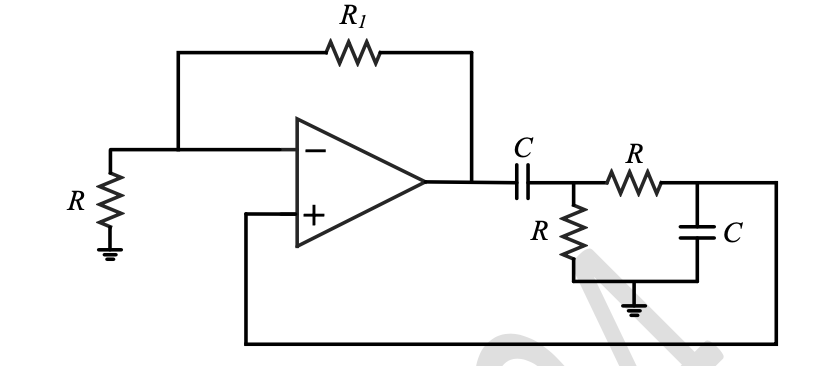
\includegraphics[width=0.5\columnwidth]{q50.png}
    \caption{For q-50}
    \label{fig:q50}
\end{figure}
\hfill{\brak{\text{GATE EC 2025}}}
\begin{multicols}{2}
\begin{enumerate}
    \item $29R$ and $1/\brak{2\pi\sqrt{6}RC}$
    \item $2R$ and $1/\brak{2\pi RC}$
    \item $29R$ and $1/\brak{2\pi RC}$
    \item $2R$ and $1/\brak{2\pi\sqrt{6}RC}$
\end{enumerate}
\end{multicols}

\item In the circuit shown in $\figref{fig:q51}$, the transistors $M_1$ and $M_2$ are biased in saturation. Their small signal transconductances are $g_{m1}$ and $g_{m2}$ respectively. Neglect body effect, channel length modulation and intrinsic device capacitances. Assuming that capacitor $C_C$ is a short circuit for AC analysis, the exact magnitude of small signal voltage gain $\abs{v_{out}/v_{in}}$ is \underline{\hspace{2cm}}.
\begin{figure}[H]
    \centering
    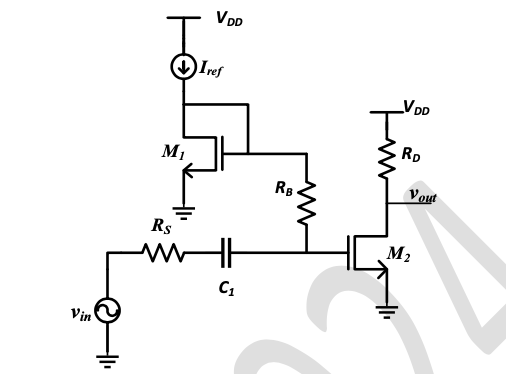
\includegraphics[width=0.3\columnwidth]{q51.png}
    \caption{for q-51}
    \label{fig:q51}
\end{figure}
\hfill{\brak{\text{GATE EC 2025}}}
\begin{multicols}{4}
    \begin{enumerate}
    \item $g_{m1}\brak{R_S || R_L}$
    \item $\dfrac{g_{m1} R_L}{1 + g_{m1} R_S}$
    \item $g_{m1} R_L$
    \item $\dfrac{g_{m1} R_L}{1 + g_{m2} R_S}$
\end{enumerate}
\end{multicols}


\item Which of the following statements is/are true for a BJT with respect to its DC current gain $\beta$?

\hfill{\brak{\text{GATE EC 2025}}}
\begin{enumerate}
    \item Under high-level injection condition in forward active mode, $\beta$ will decrease with increase in the magnitude of collector current.
    \item Under low-level injection condition in forward active mode, where the current at the emitter-base junction is dominated by recombination-generation process, $\beta$ will decrease with increase in the magnitude of collector current.
    \item $\beta$ will be lower when the BJT is in saturation region compared to when it is in active region.
    \item A higher value of $\beta$ will lead to a lower value of the collector-to-emitter breakdown voltage.
\end{enumerate}

\item Consider a system represented in state space as $\dot{x} = Ax + Bu, y = Cx + Du$. Which of the state space representations given below has/have the same transfer function as that of the original system?

\hfill{\brak{\text{GATE EC 2025}}}
\begin{enumerate}
    \item $\dot{z} = P^{-1}APz + P^{-1}Bu, y = CPz + Du$, for any invertible matrix $P$.
    \item $\dot{z} = P^{-1}APz + P^{-1}Bu, y = CPz + Du$, only if $P$ is a diagonal matrix.
    \item $\dot{z} = A^T z + C^T u, y = B^T z + D^T u$.
    \item $\dot{z} = A z + Bu, y = \brak{C+\gamma A}z + \brak{D+\gamma B}u$, for any scalar $\gamma$.
\end{enumerate}

\item Let $\vec{F} = P\hat{i} + Q\hat{j} + R\hat{k}$ be functions of $\brak{x,y,z}$. Suppose that for every given pair of points $A$ and $B$ in space, the line integral $\int_A^B \vec{F} \cdot d\vec{l}$ evaluates to the same value along any path that starts at $A$ and ends at $B$. Then which of the following is/are true?

\hfill{\brak{\text{GATE EC 2025}}}
\begin{enumerate}
    \item For every closed path $C$, we have $\oint_C \vec{F} \cdot d\vec{l} = 0$.
    \item There exists a differentiable scalar function $\phi$ such that $\vec{F} = \nabla \phi$.
    \item $\nabla \times \vec{F} = 0$.
    \item $\dfrac{\partial P}{\partial y} = \dfrac{\partial Q}{\partial x}, \dfrac{\partial Q}{\partial z} = \dfrac{\partial R}{\partial y}, \dfrac{\partial R}{\partial x} = \dfrac{\partial P}{\partial z}$.
\end{enumerate}

\item Consider the matrix $M = \myvec{1 & 0 & k \\ 0 & 1 & 0 \\ k & 0 & 1}$, where $k$ is a positive real number. Which of the following vectors is/are eigenvector(s) of this matrix?
\hfill{\brak{\text{GATE EC 2025}}}
\begin{multicols}{4}
\begin{enumerate}
    \item $\myvec{1 \\ 0 \\ -1}$
    \item $\myvec{0 \\ 1 \\ 0}$
    \item $\myvec{1 \\ 0 \\ 1}$
    \item $\myvec{k \\ 0 \\ -k}$
\end{enumerate}
\end{multicols}

\item The radian frequency value(s) for which the discrete time sinusoidal signal $x\sbrak{n} = A \cos\brak{\Omega n + \pi/3}$ has a period of 40 is/are \underline{\hspace{2cm}}.

\hfill{\brak{\text{GATE EC 2025}}}
\begin{multicols}{4}
\begin{enumerate}
    \item $0.15\pi$
    \item $0.225\pi$
    \item $0.3\pi$
    \item $0.45\pi$
\end{enumerate}
\end{multicols}

\item Let $X\brak{t} = A \cos\brak{2\pi f_0 t + \Theta}$ be a random process, where amplitude $A$ and phase $\Theta$ are independent of each other, and are uniformly distributed in the intervals $[0, 5]$ and $[0, 2\pi]$, respectively. $X\brak{t}$ is fed to an 8-bit uniform mid-rise type quantizer. Given that the autocorrelation of $X\brak{t}$ is $R_X\brak{\tau} = \dfrac{25}{2}\cos\brak{2\pi f_0 \tau}$, the signal to quantization noise ratio (in dB, rounded off to two decimal places) at the output of the quantizer is \underline{\hspace{2cm}}.

\hfill{\brak{\text{GATE EC 2025}}}

\item A lossless transmission line with characteristic impedance $Z_0 = 50 \ohm$ is terminated with an unknown load. The magnitude of the reflection co-efficient is $|\Gamma| = 0.6$. As one moves towards the generator from the load, the maximum value of the input impedance magnitude looking towards the load \brak{in $\ohm$} is \underline{\hspace{2cm}}.

\hfill{\brak{\text{GATE EC 2025}}}

\item The relationship between any N-length sequence $x\sbrak{n}$ and its corresponding N-point discrete Fourier transform $X\sbrak{k}$ is defined as $X\sbrak{k} = \mathcal{F}\{x\sbrak{n}\}$. Another sequence $y\sbrak{n}$ is formed as below $y\sbrak{n} = \mathcal{F}\{\mathcal{F}\{\mathcal{F}\{\mathcal{F}\{x\sbrak{n}\}\}\}\}$. For the sequence $x\sbrak{n} = \{1, 2, 1, 3\}$, the value of $Y\sbrak{0}$ is \underline{\hspace{2cm}}.

\hfill{\brak{\text{GATE EC 2025}}}

\item For the two port network shown in $\figref{fig:q60}$, the value of the parameter $Y_{21}$ \brak{in Siemens} is \underline{\hspace{2cm}}.
\begin{figure}[H]
    \centering
    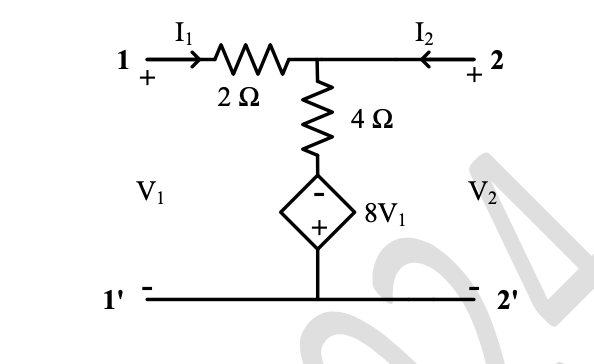
\includegraphics[width=0.5\columnwidth]{q60.png}
    \caption{For q-60}
    \label{fig:q60}
\end{figure}
\hfill{\brak{\text{GATE EC 2025}}}

\item Consider a MOS capacitor made with p-type silicon. It has an oxide thickness of 100 nm, a fixed positive oxide charge of $10^{-8}$ C/cm$^2$ at the oxide-silicon interface, and a metal work function of 4.6 eV. Assume that the relative permittivity of the oxide is 4 and the absolute permittivity of free space is $8.85 \times 10^{-14}$ F/cm. If the flatband voltage is 0 V, the work function of the p-type silicon (in eV, rounded off to two decimal places) is \underline{\hspace{2cm}}.
\hfill{\brak{\text{GATE EC 2025}}}

\item In the network shown in $\figref{fig:q62}$, maximum power is to be transferred to the load $R_L$. The value of $R_L$ \brak{in $\ohm$} is \underline{\hspace{2cm}}.
\begin{figure}[H]
    \centering
    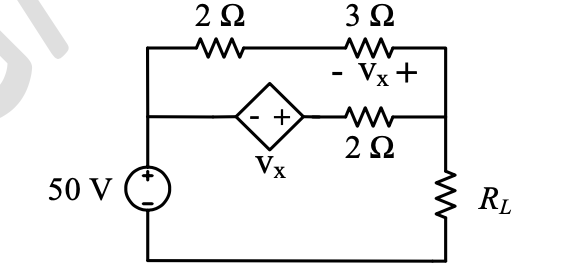
\includegraphics[width=0.5\columnwidth]{q62.png}
    \caption{For q-62}
    \label{fig:q62}
\end{figure}
\hfill{\brak{\text{GATE EC 2025}}}

\item A non-degenerate n-type semiconductor has 5 \% neutral dopant atoms. Its Fermi level is located at 0.25 eV below the conduction band \brak{$E_C$} and the donor energy level \brak{$E_D$} has a degeneracy of 2. Assuming the thermal voltage to be 20 mV, the difference between $E_C$ and $E_D$ (in eV, rounded off to two decimal places) is \underline{\hspace{2cm}}.

\hfill{\brak{\text{GATE EC 2025}}}

\item An NMOS transistor operating in the linear region has $I_{DS}$ of 5 $\mu$A at $V_{DS}$ of 0.1 V. Keeping $V_{GS}$ constant, the $V_{DS}$ is increased to 1.5 V. Given that $\mu_n C_{ox} \dfrac{W}{L}= 50 \mu\text{A/V}^2$, the transconductance at the new operating point \brak{in $\mu$A/V, rounded off to two decimal places} is \underline{\hspace{2cm}}.

\hfill{\brak{\text{GATE EC 2025}}}

\item The photocurrent of a PN junction diode solar cell is 1 mA. The voltage corresponding to its maximum power point is 0.3 V. If the thermal voltage is 30 mV, the reverse saturation current of the diode \brak{\text{in nA, rounded off to two decimal places}} is \underline{\hspace{2cm}}.

\hfill{\brak{\text{GATE EC 2025}}}


















\end{enumerate}
\end{document}